\documentclass[12pt]{article}
\usepackage[a4paper, total={5.5in, 9in}]{geometry}
\usepackage{amsmath}
\usepackage{amsfonts}
\usepackage{graphicx}
\usepackage{pgfplots} % Para crear gráficos
\pgfplotsset{compat=1.18} % Para evitar warnings de compatibilidad
\usepackage{enumitem}

\title{College Algebra Worksheet 3.1}
\author{PCL Learning Center}
\date{}

\begin{document}
\maketitle

\begin{center}
    \textit{note: No graphing calculators or electronic devices may be used on this worksheet.}    
\end{center}

\section*{Problem Set 1\\Difficulty level: Normal}
\subsection*{Problem 1}
Find the domain and range of the relation:
\[
\{(-14, -13), (-16, 17), (-17, -21), (15, -25), (-2, 13)\}
\]

\subsection*{Problem 2}
Find the value \( h(-8) \), where \( h(t) = 8t - 4 \).

\subsection*{Problem 3}
For the following exercises, evaluate \( f(-3) \), \( f(2) \), \( f(-a) \), \( -f(a) \), \( f(a+h) \).
    \begin{enumerate}
        \item \( f(x) = 2x - 5 \)
        \item \( f(x) = -5x^2 + 2x - 1 \)
        \item \( f(x) = \sqrt{2-x} + 5 \)
        \item \( f(x) = \dfrac{6x-1}{5x+2} \)
        \item \( f(x) = |x-1| - |x+1| \)
    \end{enumerate}


\subsection*{Problem 4}
Determine whether \(18x^2+6y=-18\) is a function.

\subsection*{Problem 5}
In which of the relations represented by the tables below is the output a function of the input?\\
    \begin{enumerate}
    \item[(a)]
    \begin{tabular}{|c|c|c|c|c|c|}
        \hline
        & Input & 1 & 0 & 2 & 0 \\ \hline
        & Output & 14 & 4 & 12 & 9 \\ \hline
    \end{tabular}
    
    \item[(b)]
    \begin{tabular}{|c|c|c|c|c|c|}
        \hline
        & Input & \(-4\) & \(-4\) & 3 & \(-1\) \\ \hline
        & Output & \(-5\) & 13 & \(-1\) & \(-3\) \\ \hline
    \end{tabular}
    
    \item[(c)]
    \begin{tabular}{|c|c|c|c|c|c|}
        \hline
        & Input & 5 & 6 & 7 & 4 \\ \hline
        & Output & 2 & 1 & 3 & 2 \\ \hline
    \end{tabular}
    
    \item[(d)]
    \begin{tabular}{|c|c|c|c|c|c|}
        \hline
        & Input & 2 & \(-2\) & \(-1\) & \(-3\) \\ \hline
        & Output & 2 & 1 & 8 & 8 \\ \hline
    \end{tabular}
    
    \item[(e)]
    \begin{tabular}{|c|c|c|c|c|c|}
        \hline
        & Input & 2 & \(-1\) & 2 & \(-3\) \\ \hline
        & Output & 10 & 2 & 1 & 3 \\ \hline
    \end{tabular}
    \end{enumerate}
\subsection*{Problem 6}
Given the following table of values for \(f(x)\), find \( f(9) \).
    \[
    \begin{array}{|c|c|c|c|c|c|c|} % 7 columnas (x + 6 valores)
    \hline
    x & -4 & -3 & -1 & 5 & 7 & 9 \\ 
    \hline
    f(x) & 3 & 0 & 9 & 13 & 1 & 1 \\ 
    \hline
    \end{array}
    \]

\subsection*{Problem 7}
Why does the vertical line test tell us whether the graph of a relation represents a function? Please elaborate.

\subsection*{Problem 8}
Given the table below, determine whether \( y \) is a function of \( x \) and whether it is one-to-one.

    \begin{center}
    \begin{tabular}{|c|c|}
    \hline
    \( x \) & \( y \) \\
    \hline
    6    & 3    \\
    1    & 2    \\
    3    & 12   \\
    9    & 3    \\
    7    & 9    \\
    \hline
    \end{tabular}
    \end{center}

    \begin{enumerate}
        \item[(a)] \( y \) is not a function of \( x \).
        \item[(b)] \( y \) is a function of \( x \), and the function is one-to-one.
        \item[(c)] \( y \) is a function of \( x \), but the function is not one-to-one.
    \end{enumerate}
\subsection*{Problem 9}
Which of the following graphs show a one-to-one function?

\begin{enumerate}[label=(\alph*)]
    \item 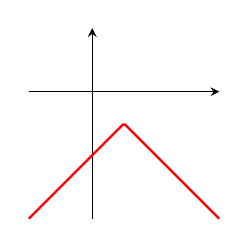
\begin{tikzpicture}
        \begin{axis}[
            axis lines=middle,
            xtick=\empty, ytick=\empty,
            width=4cm,
            height=4cm,
            xmin=-2, xmax=4,
            ymin=-4, ymax=2,
            clip=false
        ]
        \addplot[red, thick, domain=-2:4, samples=100] {-abs(x - 1) - 1};
        \end{axis}
    \end{tikzpicture}
    
    \item 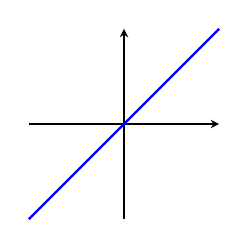
\begin{tikzpicture}
        \begin{axis}[
            axis lines=middle,
            xtick=\empty, ytick=\empty,
            width=4cm,
            height=4cm,
            xmin=-4, xmax=4,
            ymin=-2, ymax=2,
            clip=false
        ]
        \addplot[blue, thick, domain=-4:4, samples=100] {x/2};
        \end{axis}
    \end{tikzpicture}
    
    \item 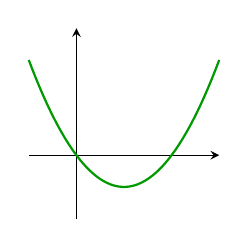
\begin{tikzpicture}
        \begin{axis}[
            axis lines=middle,
            xtick=\empty, ytick=\empty,
            width=4cm,
            height=4cm,
            xmin=-1, xmax=3,
            ymin=-2, ymax=4,
            clip=false
        ]
        \addplot[green!60!black, thick, domain=-1:3, samples=100] {(x - 1)^2 - 1};
        \end{axis}
    \end{tikzpicture}
    
    \item 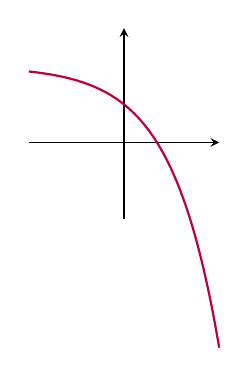
\begin{tikzpicture}
        \begin{axis}[
            axis lines=middle,
            xtick=\empty, ytick=\empty,
            width=4cm,
            height=4cm,
            xmin=-2, xmax=2,
            ymin=-2, ymax=3,
            clip=false
        ]
        \addplot[purple, thick, domain=-2:2, samples=100] {-exp(x) + 2};
        \end{axis}
    \end{tikzpicture}
\end{enumerate}


\subsection*{Problem 10}
Given the graph of \( y = f(x) \), solve for \( f(x) = 4 \).

    \begin{center}
    \begin{tikzpicture}
    \begin{axis}[
        axis lines=middle,
        width=10cm,
        height=8cm,
        xmin=-2, xmax=6,
        ymin=-1, ymax=6,
    ]
    \addplot[red, thick, domain=-2:6, samples=100] {(x - 2)^2};
    \end{axis}
    \end{tikzpicture}
    \end{center}



\subsection*{Problem 11}
Given the following function, solve for \(h(y)=1\).
\[ h(y)=\sqrt[13]{3y-8}\]

\subsection*{Problem 12}
Which of the following graphs show a function?


\begin{enumerate}[label=(\alph*)]
    % (a) parabola rotada a la derecha
    \item 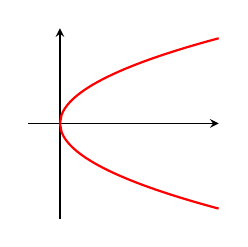
\begin{tikzpicture}
        \begin{axis}[
            axis lines=middle,
            xtick=\empty, ytick=\empty,
            width=4cm,
            height=4cm,
            xmin=-1, xmax=5,
            ymin=-2.5, ymax=2.5,
            clip=false
        ]
        \addplot[red, thick, domain=0:5, samples=100] {sqrt(x)};
        \addplot[red, thick, domain=0:5, samples=100] {-sqrt(x)};
        \end{axis}
    \end{tikzpicture}


    % (b) valor absoluto rotado a la izquierda
    \item \begin{tikzpicture}
        \begin{axis}[
            axis lines=middle,
            xtick=\empty, ytick=\empty,
            width=4cm,
            height=4cm,
            xmin=-6, xmax=2,
            ymin=-4, ymax=4,
            clip=false
        ]
        \addplot[blue, thick, domain=-4:4, samples=100] {-abs(x) - 2}; % x = -|y| - 2
        \end{axis}
    \end{tikzpicture}

    % (c) log(x)
    \item 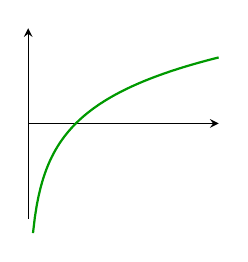
\begin{tikzpicture}
        \begin{axis}[
            axis lines=middle,
            xtick=\empty, ytick=\empty,
            width=4cm,
            height=4cm,
            xmin=0, xmax=4,
            ymin=-2, ymax=2,
            clip=false
        ]
        \addplot[green!60!black, thick, domain=0.1:4, samples=100] {ln(x)};
        \end{axis}
    \end{tikzpicture}

    % (d) parabola normal (x-2)^2 - 2
    \item 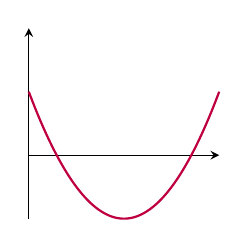
\begin{tikzpicture}
        \begin{axis}[
            axis lines=middle,
            xtick=\empty, ytick=\empty,
            width=4cm,
            height=4cm,
            xmin=0, xmax=4,
            ymin=-2, ymax=4,
            clip=false
        ]
        \addplot[purple, thick, domain=0:4, samples=100] {(x - 2)^2 - 2};
        \end{axis}
    \end{tikzpicture}
\end{enumerate}

\subsection*{Problem 13}
What is the difference between the input and the output of a function?

\section*{Problem Set 2\\Difficulty level: Hard}
\subsection*{Problem 1}
Given the function \(\phi(x)=x^2+2x\), evaluate
\[\dfrac{\phi(x)-\phi(a)}{x-a} \text{, where } x \not= a.\]


\newpage
\section*{Solutions to the Set 1}
\subsection*{Problem 1}
domain: \(\{-17,-16,-14,-2,15\}\), range: \(\{-25,-21,-13,13,17\}\)
\subsection*{Problem 2}
\(h(-8)=-68\)
\subsection*{Problem 3}
\begin{enumerate}
    \item \( f(x) = 2x - 5 \).\\
    \( f(-3) = -11 \), \hspace{0.7cm} \( f(2) = -1 \), \hspace{0.7cm} \( f(-a) = -2a - 5 \),\\
    \( -f(a) = -2a + 5 \), \hspace{0.7cm} \( f(a+h) = 2(a+h) - 5 \).

    \item \( f(x) = -5x^2 + 2x - 1 \).\\
    \( f(-3) = -52 \), \hspace{0.7cm} \( f(2) = -17 \), \hspace{0.7cm} \( f(-a) = -5a^2 - 2a - 1 \),\\
    \( -f(a) = 5a^2 - 2a + 1 \), \hspace{0.7cm} \( f(a+h) = -5(a+h)^2 + 2(a+h) - 1 \).

    \item \( f(x) = \sqrt{2-x} + 5 \).\\
    \( f(-3) = \sqrt{5} + 5 \), \hspace{0.7cm} \( f(2) = 5 \), \hspace{0.7cm} \( f(-a) = \sqrt{2 + a} + 5 \),\\
    \( -f(a) = -\sqrt{2 - a} - 5 \),\hspace{0.7cm} \( f(a+h) = \sqrt{2 - (a+h)} + 5 \).

    \item \( f(x) = \dfrac{6x-1}{5x+2} \).\\ 
    \( f(-3) = \dfrac{19}{13} \),\hspace{0.7cm} \( f(2) = \dfrac{11}{12} \),\hspace{0.7cm} \( f(-a) = \dfrac{-6a - 1}{-5a + 2} \),\\
    \( -f(a) = \dfrac{-6a + 1}{5a + 2} \),\hspace{0.7cm} \( f(a+h) = \dfrac{6(a+h) - 1}{5(a+h) + 2} \).

    \item \( f(x) = |x - 1| - |x + 1| \).\\ 
    \( f(-3) = 2 \), \hspace{0.7cm}\( f(2) = -2 \),\hspace{0.7cm} \( f(-a) = | -a - 1 | - | -a + 1 | \),\\
    \( -f(a) = -|a - 1| + |a + 1|) \),\hspace{0.7cm} \( f(a+h) = |(a+h) - 1| - |(a+h) + 1| \).
\end{enumerate}
\subsection*{Problem 4}
Yes.
\subsection*{Problem 5}
\begin{enumerate}
    \item[(c)]
    \item[(d)]
\end{enumerate}
\subsection*{Problem 6}
\(f(9)=1\)
\subsection*{Problem 7}
We need to recall that a function can assign only one output for each input. With that in mind, if a vertical line intersects the graph at more than one point, it means that a single input \(x\) is mapped to multiple outputs, which of course violates the principle of what is a function.
\subsection*{Problem 8}
\begin{enumerate}
    \item[(c)] \( y \) is a function of \( x \), but the function is not one-to-one.
\end{enumerate}
\subsection*{Problem 9}
\begin{enumerate}
    \item[(b)]
    \item[(d)] 
\end{enumerate}
\subsection*{Problem 10}
\(x=0\) and \(x=4\)
\subsection*{Problem 11}
\(y=3\)
\subsection*{Problem 12}
\begin{enumerate}
    \item[(a)]
    \item[(b)]
    \item[(c)]
\end{enumerate}
\subsection*{Problem 13}
The input of a function is the value we provide, usually denoted as \(x\), and the output is the result the function gives, usually denoted as \(f(x)\). 

\section*{Solutions to the Set 2}
\subsection*{Problem 1}
\(x+a+2\)

\end{document}

